\chapter{Results}
\label{chap:results}
The desired results in this project thesis are confirmation that the two models are working and are ready to be used in the master thesis. 
\section{Results from Testing of Global Model}
The static configuration for the three different wind conditions: 
\begin{figure}[H]
\subfloat[Near position\label{fig:cavS200}]
  {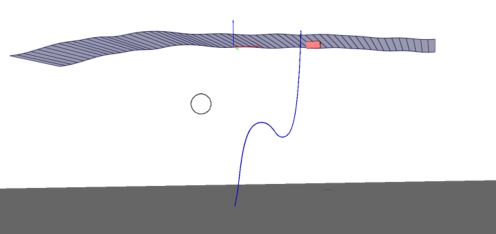
\includegraphics[width=.3\linewidth]{figures/staposnear}}\hfill
\subfloat[Neutral position \label{fig:cavS2500}]
  {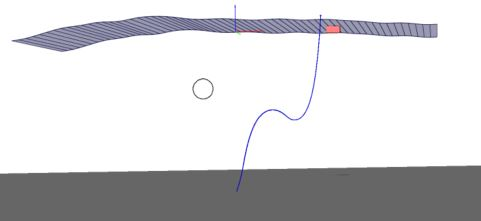
\includegraphics[width=.3\linewidth]{figures/statposneu}}\hfill
  \subfloat[Far position \label{fig:cavS5000}]
  {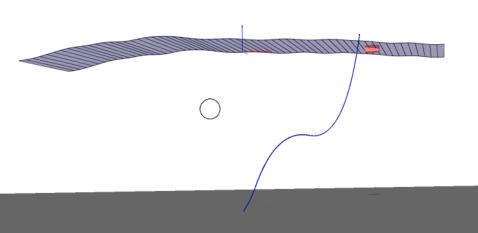
\includegraphics[width=.3\linewidth]{figures/statposfar}}\hfill
\caption{Static configuration for the global model for different wind conditions}
\label{fig:statcon}
\end{figure}

\noindent These positions gave the following configurations for the dynamic cable: 
\begin{figure}[H]
\centering
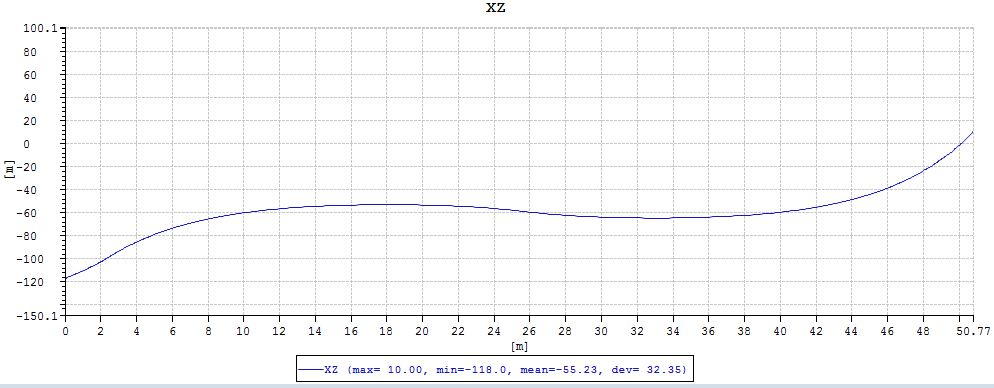
\includegraphics[scale=0.5]{figures/confignear}
\caption{Configuration for near position}
 \label{fig:confignear}
\end{figure}

\begin{figure}[H]
\centering
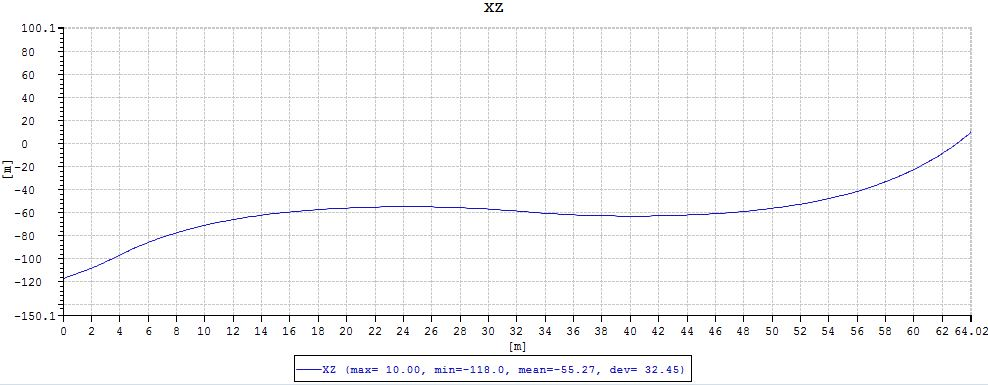
\includegraphics[scale=0.5]{figures/configneu}
\caption{Configuration for neutral position}
 \label{fig:configneu}
\end{figure}

\begin{figure}[H]
\centering
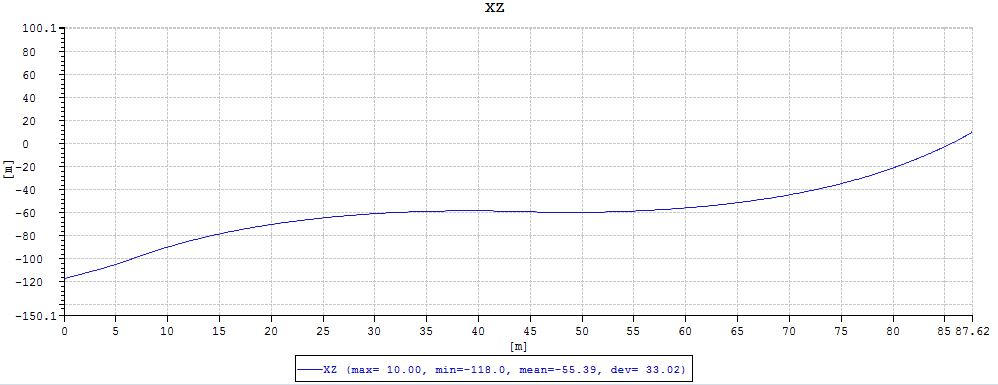
\includegraphics[scale=0.5]{figures/configfar}
\caption{Configuration for far position}
 \label{fig:configfar}
\end{figure}

\noindent The envelope curves for the curvatures

\begin{figure}[H]
\centering
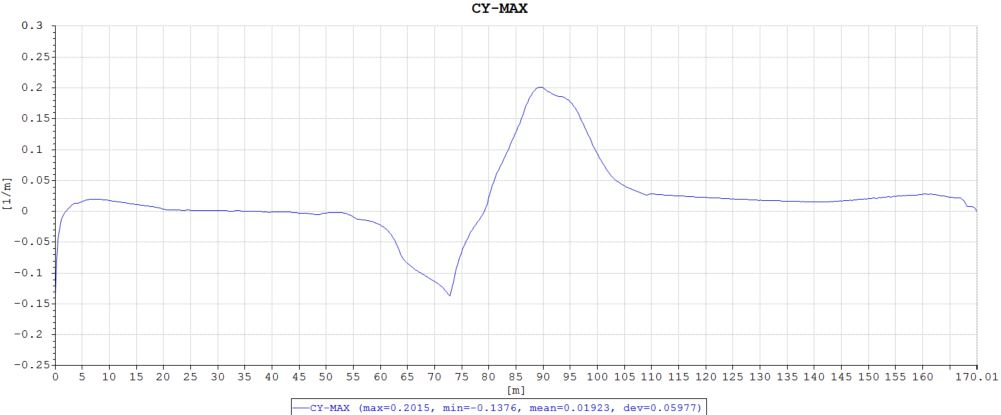
\includegraphics[scale=0.8]{figures/envcurvenear}
\caption{Curvature envelope for near position}
 \label{fig:envcurvenear}
\end{figure}

\begin{figure}[H]
\centering
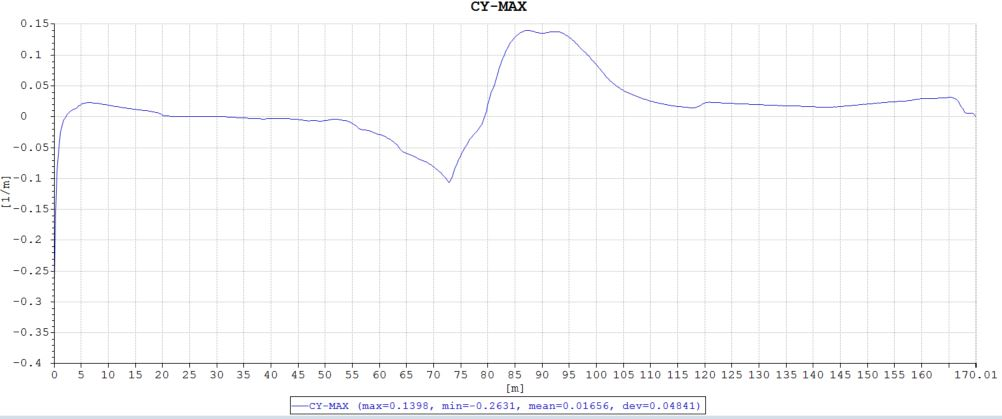
\includegraphics[scale=0.8]{figures/envcurveneu}
\caption{Curvature envelope for neutral position}
 \label{fig:envcurveneu}
\end{figure}

\begin{figure}[H]
\centering
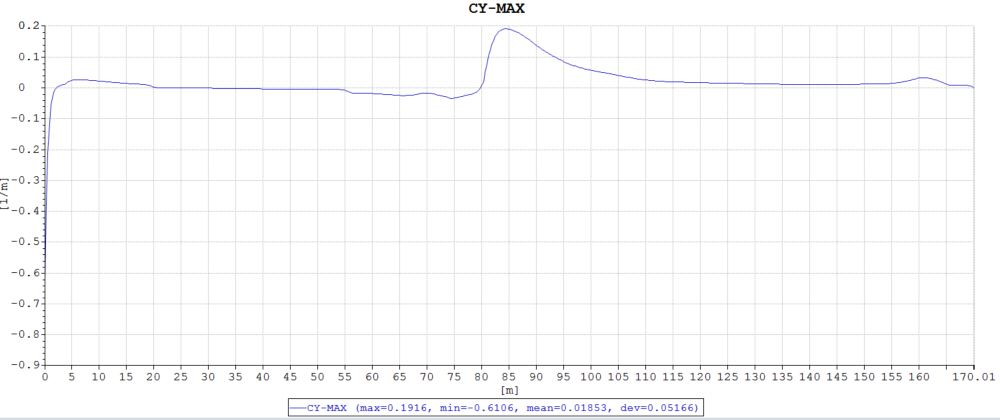
\includegraphics[scale=0.8]{figures/envcurvefar}
\caption{Curvature envelope for far position}
 \label{fig:envcurvefar}
\end{figure}

\noindent The max tension over the length of the cable

\begin{figure}[H]
\centering
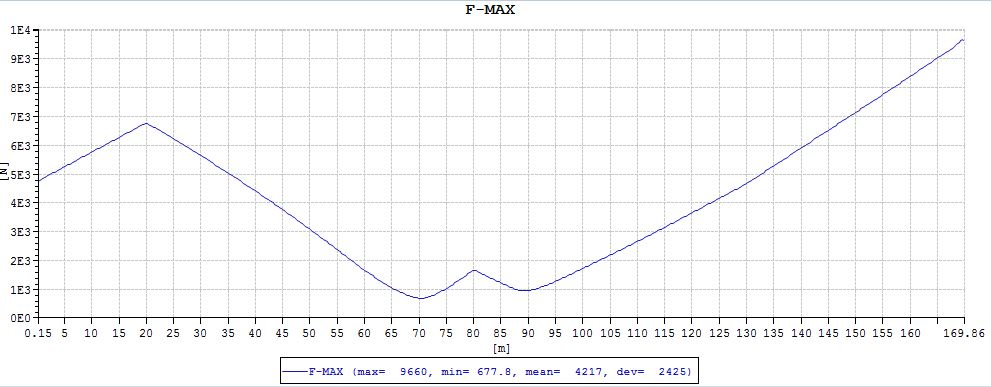
\includegraphics[scale=0.5]{figures/fmaxnear}
\caption{The max tension over the length of the cable in near position}
 \label{fig:fmaxnear}
\end{figure}


\begin{figure}[H]
\centering
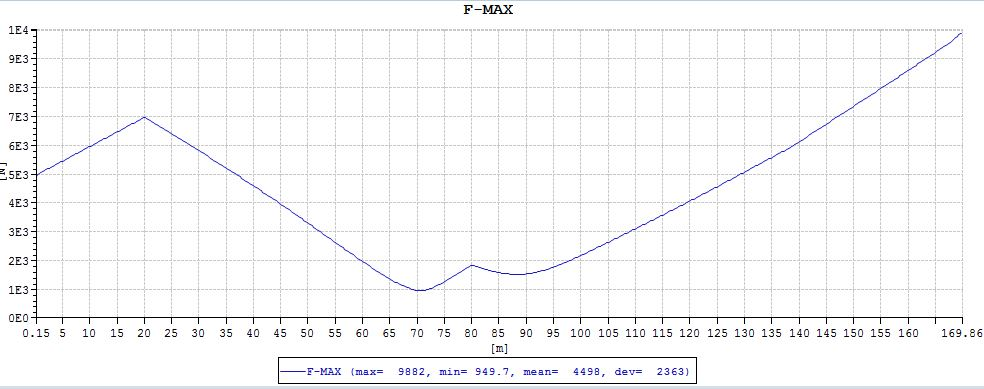
\includegraphics[scale=0.5]{figures/fmaxneu}
\caption{The max tension over the length of the cable in neutral position}
 \label{fig:fmaxneu}
\end{figure}


\begin{figure}[H]
\centering
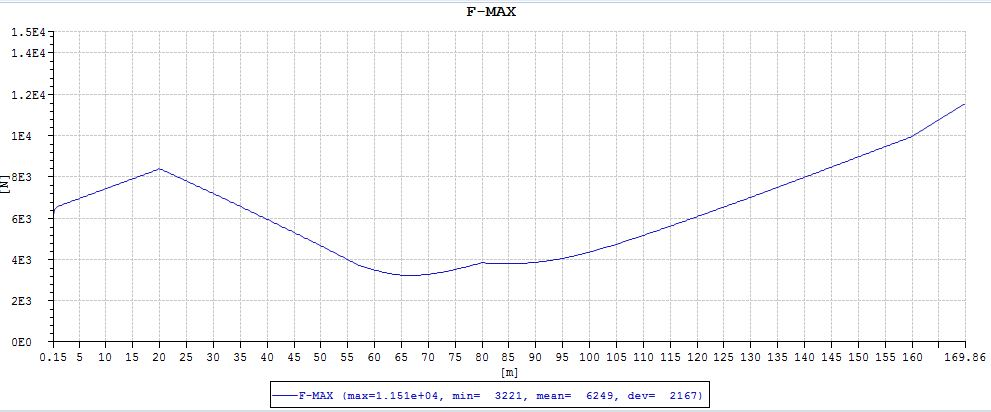
\includegraphics[scale=0.5]{figures/fmaxfar}
\caption{The max tension over the length of the cable in far position}
 \label{fig:fmaxfar}
\end{figure}

\noindent The minimum tension over the length of the cable

\begin{figure}[H]
\centering
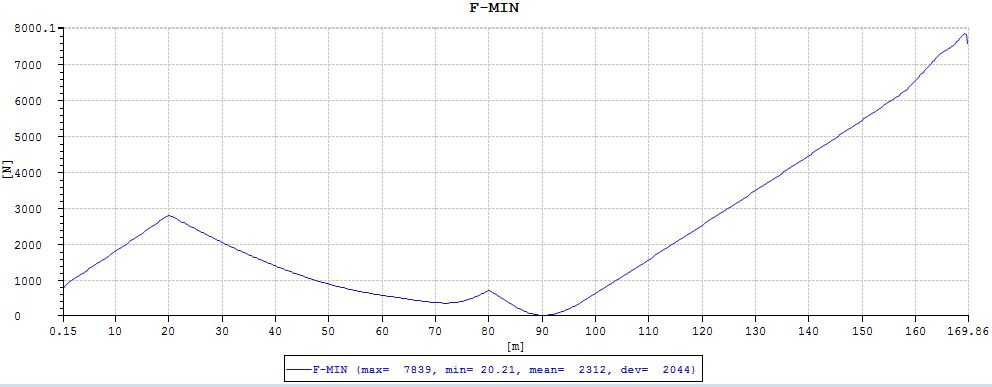
\includegraphics[scale=0.5]{figures/fminnear}
\caption{The minimum tension over the length of the cable in near position}
 \label{fig:fminnear}
\end{figure}


\begin{figure}[H]
\centering
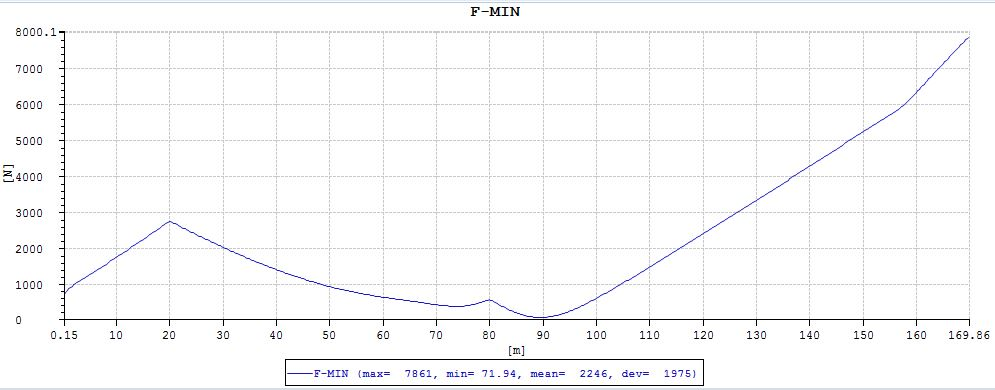
\includegraphics[scale=0.5]{figures/fminneu}
\caption{The minimum tension over the length of the cable in neutral position}
 \label{fig:fminneu}
\end{figure}


\begin{figure}[H]
\centering
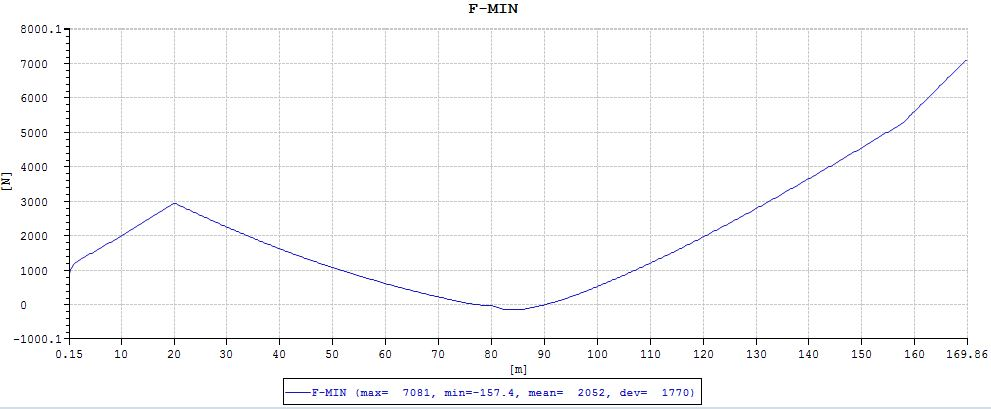
\includegraphics[scale=0.5]{figures/fminfar}
\caption{The minimum tension over the length of the cable in far position}
 \label{fig:fminfar}
\end{figure}

\section{Local Model}
The following figures show the local model and some of its components:

\begin{figure}[H]
\subfloat[Local model from the side with bend stiffener \label{fig:lm_total}]
  {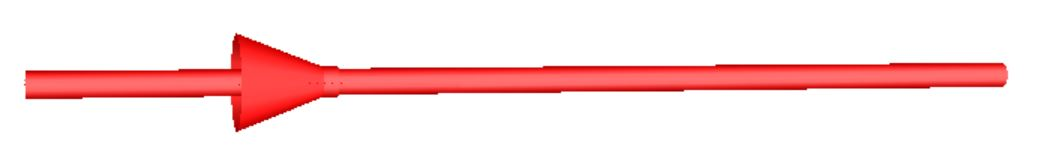
\includegraphics[width=.45\linewidth]{figures/lm_total}}\hfill
\subfloat[Cable cross section in local model \label{fig:lm_cross}]
  {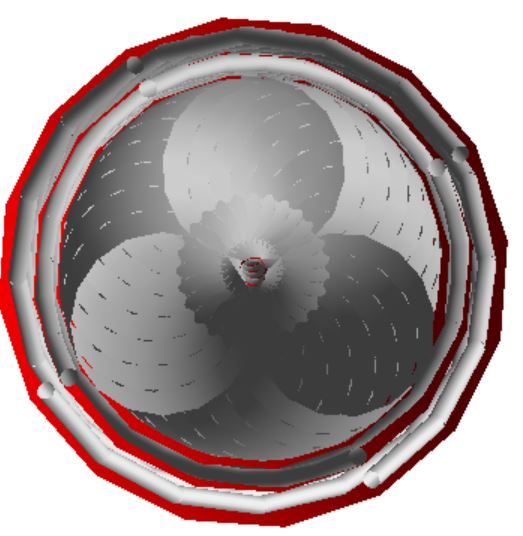
\includegraphics[width=.25\linewidth]{figures/lm_cross}}\hfill
\caption{Local model}
\label{fig:volt}
\end{figure}

\begin{figure}[H]
\subfloat[Conductors \label{fig:single}]
  {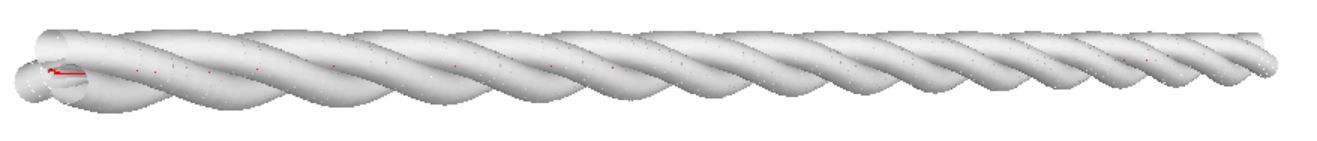
\includegraphics[width=.45\linewidth]{figures/lm_conductors}}\hfill
\subfloat[Armouring \label{fig:3phase}]
  {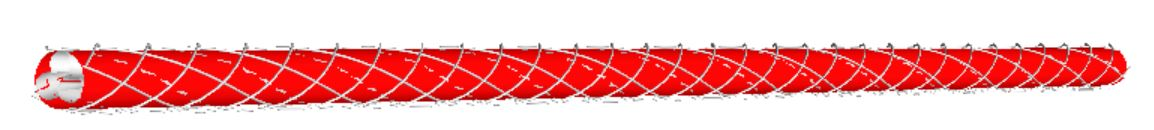
\includegraphics[width=.45\linewidth]{figures/lm_arm}}\hfill
\caption{Helical components in the local model}
\label{fig:volt}
\end{figure}
